\chapter{Software Defined Radio and GNU Radio Framework}\label{sec:sdrgnur}

In this chapter a general introduction to the \gls{sdr} concept is given. Additionally, advantages of SDRs and given hardware limitations are addressed. Here, the GNU Radio SDR framework is presented giving insight into the basic architectural features.

An \gls{sdr} is a radio that is built entirely or in large parts in software, which runs on a general purpose computer. A more extensive definition is given by Joseph Mitola, who established the term Software Radio~\cite{Mitola200609}:

\say{A software radio is a radio whose channel modulation waveforms are defined in software. That is, waveforms are generated as sampled digital signals, converted from digital to analog via a wideband \gls{dac} and then possibly upconverted from \gls{if} to \gls{rf}. The receiver, similarly, employs a wideband \gls{adc} that captures all of the channels of the software radio node. The receiver then extracts, downconverts and demodulates the channel waveform using software on a general purpose processor. Software radios employ a combination of techniques that include multi-band antennas and \gls{rf} conversion; wideband \gls{adc} and \gls{dac}; and the implementation of \gls{if}, baseband and bitstream processing functions in general purpose programmable processors. The resulting software defined radio (or software radio) in part extends the evolution of programmable hardware, increasing flexibility via increased programmability.}


This means, that instead of using analog circuits or a specialized \gls{dsp} to process radio signals, the digitized signals are processed by architecture independent, and high level software running on general purpose processors. The term radio designates any device, that transmits and/or receives radio waves. While most modern radios contain firmware that is written in some kind of programming language, the important distinction in a software radio is that it is not tailored to a specific chip or platform, and it is therefore possible to reuse its code across different underlying architectures~\cite{DABETH}.

\section{Ideal Software Defined Radio and Practical Limitations}\label{sec:sdr}

In the ideal case, the only hardware that is needed besides a computer is an antenna and an \gls{adc} for the receiver, as well as a \gls{dac} for the transmitter. An \gls{sdr} would thus look as depicted in {~\cref{fig:idealsdr}}. In the receiver, a transmitted radio signal is picked up by an antenna, and then fed into an \gls{adc} to sample it. Once digitized, the signal is sent to some general purpose computer (e.g. an embedded PC) for processing. The transmitter looks very similar, except that the signal is sent in the reverse direction, and a \gls{dac} is used instead of an \gls{adc}. In a complete transceiver, the processing unit and the antenna may be shared between receiver and transmitter.

While the approach presented in the previous section is very simple and (in the ideal case) extremely versatile, it is not practical, due to limitations in real hardware. However, various solutions have been suggested to overcome these problems. A quick look at the different hardware limitations is given below. For better readability, only the receiving side is discussed. The transmitting side is constructed symmetrically.
%
\begin{figure}[thb]
\centering
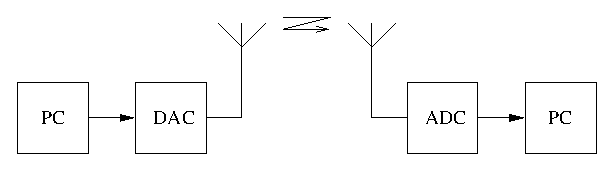
\includegraphics[width=0.6\linewidth]{idealsdr.eps}
\caption{Ideal SDR transmission\label{fig:idealsdr}}
\end{figure}
%
\begin{itemize}
 \item \textit{\Acrlong{adc}}: According to the Nyquist sampling theorem, the sampling rate of the \glspl{adc}  must be at least twice as high as the bandwidth of received signal which limits the maximum bandwidth of the received signal. Conventional \glspl{adc} are capable of sampling rates in the area of \SI{500}{Msps}, which translates to a bandwidth of \SI{250}{\mega\hertz}. While this bandwidth is enough for most current applications, the carrier frequency is usually higher than \SI{250}{\mega\hertz}. In practice, a \gls{rf} frontend is therefore usually required, to convert the received signal to an \gls{if}. Notably, as of 2018 there exists 12-bit \glspl{adc} which can sample at \SI{6.4}{\giga s\per\second}. This allows to directly digitize\footnote{Therefore it is often called direct-RF sampling.} signals at \gls{rf} frequencies and achieve sufficient dynamic range for modern communications. However, this technology is costly and not energy-efficient.
 
The second parameter, the \gls{adc} resolution influences the dynamic range of the receiver. As each additional bit doubles the resolution of the sampled input voltage, the dynamic range can be roughly estimated as $R = 6dB \times n$ where $R$ is the dynamic range and $n$ the number of bits in the \gls{adc}. As \glspl{adc} used for \gls{sdr} usually have a resolution of less than 16 bits, it is important to filter out strong interfering signals, such as signals from mobile phones, before the wideband \glspl{adc}. This is usually done in the \gls{rf} frontend. 

\item \textit{Bus Speed}: Another problem lies in getting the data from the \gls{adc} to the computer. For any practical bus, there is a maximum for the possible data rate, limiting the product of sample rate and resolution of the samples. The speed of common buses in commodity PCs ranges from a few Mbps to several Gbps as an example, the \gls{pcie} Gen~5 bus has a theoretical maximum speed of \SI{64}{\giga\byte\per\second} (in one direction). However, the speed is limited by the connections on your PC. For USB-C has a theoretical transfer speed of \SI{20}{\giga\bit\per\second}, which would not support transfering direct-\gls{rf} samples. 

\item \textit{Performance of the Processing Unit}: For real-time processing, the performance of the \gls{cpu} and the sample rate limit the number of mathematical operations that can be performed per sample, as samples must be processed as fast as they arrive. In practice, this means that fast \glspl{cpu}, clever programming and possibly parallelization is needed. If this does not suffice, a compromise must be found, to use a less optimal but faster signal processing algorithm.

\item \textit{Latency}: Since general purpose computers are not designed for real-time applications, a rather high latency can occur in practical \glspl{sdr}. While latency is not much of an issue in transmit-only or receive-only applications, many wireless standards, such as \gls{lte} require precise timing, and are therefore very difficult to implement in an \gls{sdr}.
\end{itemize}

Hence, we need to reduce the number of samples. This is done by first down-converting the analog \gls{rf} signal to an \acrlong{if} (superheterofyne receiver) or directly to baseband and perform quadrature sampling  (direct conversion or zero-IF). 

\begin{figure}[hbtp]
    \centering
    \begin{subfigure}[b]{0.32\textwidth}
         \centering
         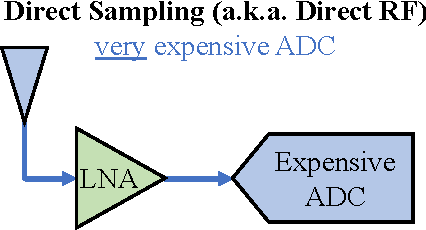
\includegraphics[width=0.9\textwidth]{figs/direct-rf.pdf}
         \caption{Direct RF}
         \label{fig:direct-rf}
     \end{subfigure}
     \hfill
     \begin{subfigure}[b]{0.32\textwidth}
         \centering
         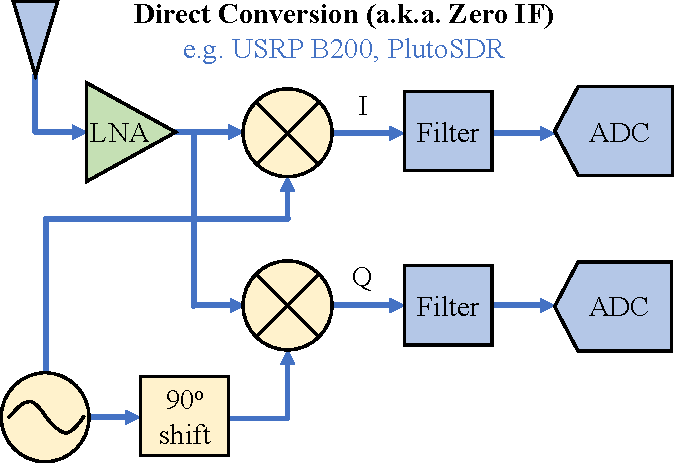
\includegraphics[width=0.9\textwidth]{figs/zero-if.pdf}
         \caption{Zero IF}
         \label{fig:zero-if}
     \end{subfigure}
     \hfill
     \begin{subfigure}[b]{0.32\textwidth}
         \centering
         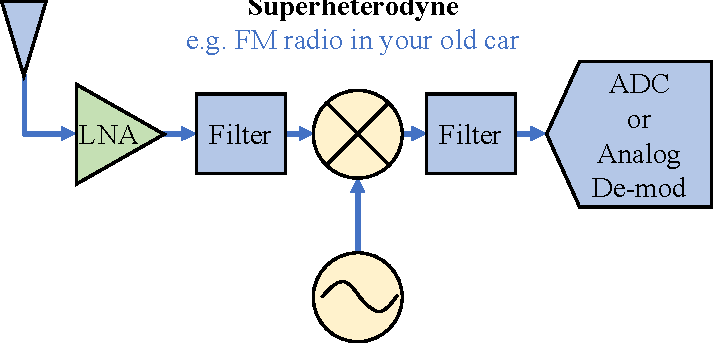
\includegraphics[width=0.9\textwidth]{figs/superheterodyne.pdf}
         \caption{Superheterodyne}
         \label{fig:superheterodyne}
     \end{subfigure}
    \caption{RF Architectures (from \url{pysdr.org})}
    \label{fig:rf-arch}
\end{figure}

Because of the use of general purpose processing units, an implementation of a given wireless
application as an \gls{sdr} is likely to use more power and occupy more space than a hardware radio
with analog filtering and possibly a dedicated signal processor. Because an \gls{sdr} contains more
complex components than a hardware radio, it will likely be more expensive, given a large
enough production volume.

Nevertheless, \gls{sdr} concepts carry the flexibility of software over to the radio world and introduces a number of interesting possibilities.
For example, very much the same way as someone may load an alternative word processor or Internet
browser on a PC, depending on the task at hand, a \gls{sdr} could allow its user to load a different
configuration, depending on whether the user wants to listen to a broadcast radio transmission,
place a phone call or determine the position via \gls{gps}.%A new
%application may even be added after the device is finished. 
Since the same hardware can be used
for any application, a great reuse of resources is possible. Another interesting possibility enabled by \gls{sdr} is the creation of a cognitive radio, which is
aware of its \gls{rf} environment and adapts itself to changes in the environment. By doing this,
a cognitive radio can use both the \gls{rf} spectrum and its own energy resources more efficiently.
As a cognitive radio requires a very high degree of flexibility, the concept of \gls{sdr} is very convenient for its practical realization.

\section{GNU Radio Architecture}\label{sec:gnur}

GNU~Radio is an open source, free software toolkit for building \glspl{sdr} \cite{GNUR}. It is designed to run on commodity computers combined with minimal hardware, allowing the construction of simple software radios \cite{DABETH}. The project was started in early 2000 by Eric Blossom and has evolved into a mature software infrastructure that is used by a large community of developers. It is licensed under the \gls{gpl}, thus anyone is allowed to use, copy and modify GNU~Radio without limits, provided that extensions are made available under the same license. While GNU~Radio was initially started on a Linux platform, it now supports various Windows, MAC and various Unix platforms.

GNU~Radio architecture consists of two components. The first component is the set of numerous building blocks which represents \Cpp\ implementations of digital signal processing routines such as (de)modulation, filtering, (de)coding and I/O operations such as file access, for further information about \Cpp\ programming see for example~\cite{Meyers,Meyers2,Meyers3,Stroustrup,Sutter}. The second component is a framework to control the data flow among blocks, implemented as Python scripts enabling easy reconfiguration and control of various system functionalities and parameters, for further studies on Python see e.g.,~\cite{Martelli}. By \textit{wiring} together such building blocks, a user can create a software defined radio, similar to connecting physical \gls{rf} building blocks to create a hardware radio. An \gls{rf} interface for GNU~Radio architecture is realized by \gls{usrp} boards, a general purpose \gls{rf} hardware, which performs computationally intensive operations as filtering, up- and down-conversion. The \gls{usrp} B210s connected via USB, which we will be using in this lab, are controlled through a robust \gls{api} provided by GNU~Radio.\footnote{Note that the \glspl{usrp} can also be programmed with the UHD library from Ettus. This provides a more low-level access to the device, and is therefore out of scope of this lab.}
\subsection{Gnu Radio Framework}
A data flow among different blocks is abstracted by \textbf{flowgraph}, a directed acyclic graph in which the vertices are the GNU~Radio blocks and the edges corresponds to data \textbf{streams}, as shown in ~\cref{flowgraph}. 
%
\begin{figure}[thb]
\centering
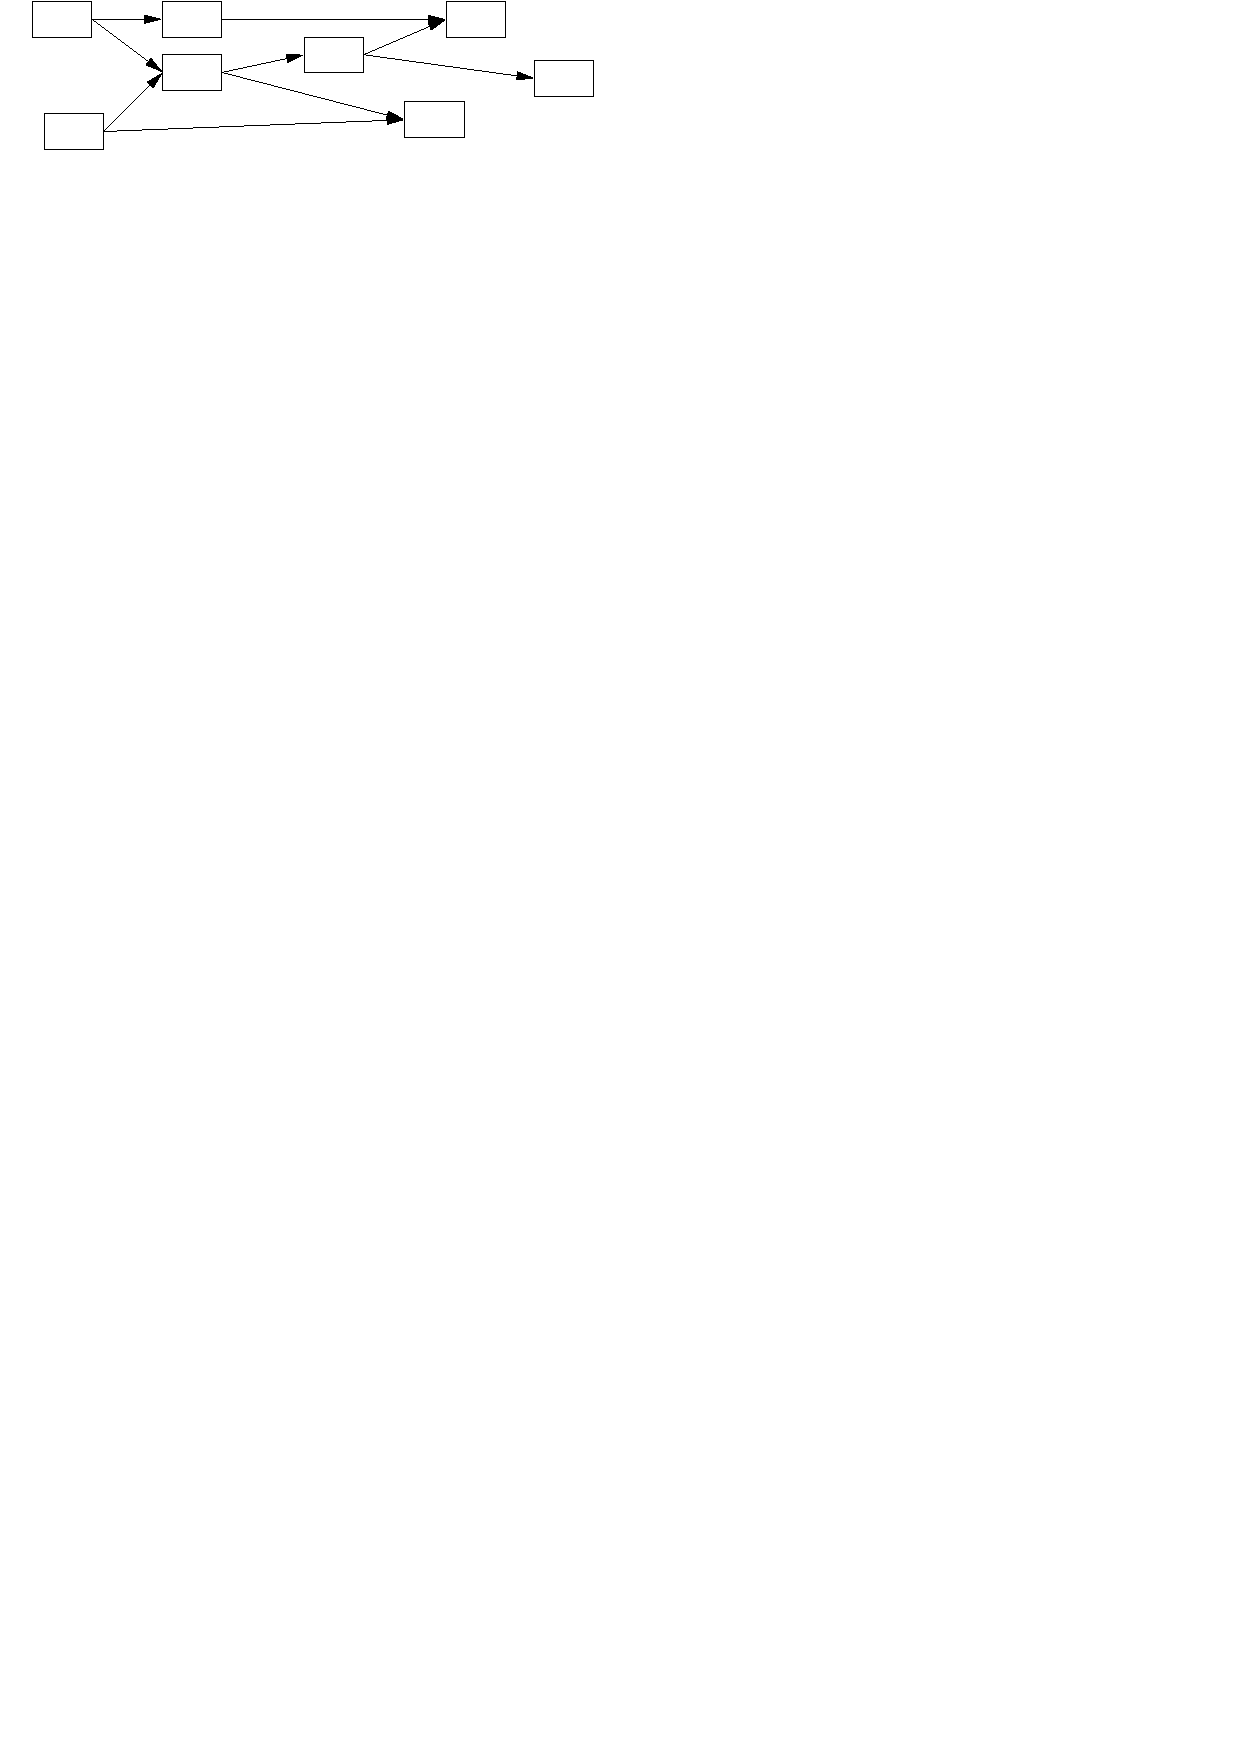
\includegraphics{gr_graph_example}
\caption{An example of \textbf{flowgraph}}\label{flowgraph}
\end{figure}
%
Generally, GNU~Radio blocks, shown in ~\cref{fig:gnuradio_block} operate on continuous streams of data. Most blocks have a set of input and/or output ports, therefore, they consume data from input streams and generate data for their output streams. Special blocks called sources and sinks only consume or produce data, respectively. Examples of sources and sinks are blocks that read and write, respectively, from \gls{usrp} receive ports, sockets, and file descriptors. Each block has an input and output signature (IO signatures) that defines the minimum and maximum number of input and output streams it can have, as well as the size of the data type on the corresponding stream. Examples of supported types are
\begin{itemize}
 \item \texttt{c} - complex interleaved floats (8 byte each),
\item \texttt{f} - floats (4 byte),
\item \texttt{s} - short integers (2 byte) and
\item \texttt{b} - byte integers (1 byte).
\end{itemize}
%
\begin{figure}[thb]
\centering
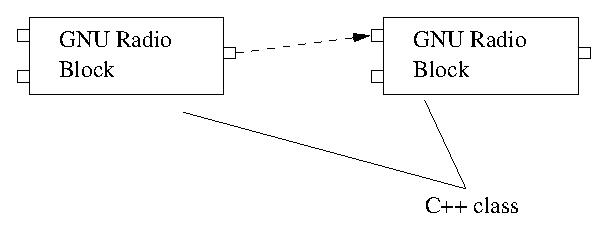
\includegraphics{gr_blocks.eps}
\caption{GNU Radio blocks}\label{fig:gnuradio_block}
\end{figure}

A full list of the supported data types can be found in GNU Radio Companion by clicking on \texttt{Help~>~Types}.
%

Each block defines a \textbf{general\_work()} function that operates on its input to produce output streams. In order to help the scheduler decide when to call the work function, blocks also provide a \textbf{forecast()} function that returns the system runtime, the number of input items it requires to produce a number of output items and how many output items it can produce given a number of input items. At runtime, blocks tell the system how many input (output) items they consumed (produced). Blocks may consume data on each input stream at a different rate, but all output streams must produce data at the same rate. The input and output streams of a block have buffers associated with them. Each input stream has a read buffer, from which the block reads data for processing. Similarly, after processing, blocks write data to the appropriate write buffers of its output streams. The data buffers are used to implement the edges in the flowgraph: the input buffers for a block are the output buffers of the upstream block in the flowgraph. GNU~Radio buffers are single writer, multiple reader FIFO (First in First Out) buffers.
%
\begin{figure}[thb]
\centering
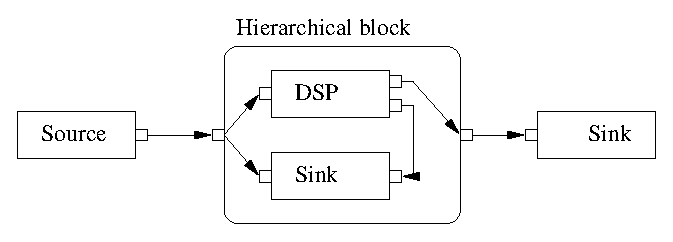
\includegraphics{hier_flowgraph.eps}
\caption{An example of a flowgraph with a hierarchical block}\label{fig:hier_flowgraph}
\end{figure}
%
Several blocks are connected in Python\index{Python} forming a flowgraph using the \textbf{connect} function which specifies how the output stream(s) of a processing block connects to the input stream of one or more downstream blocks. The flowgraph mechanism then automatically builds the flowgraph; the details of this process are hidden from the user. A key function during flowgraph construction is the allocation of data buffers to connect neighboring blocks. The buffer allocation algorithm considers the input and output block sizes used by blocks and the relative rate at which blocks consume and produce items on their input and output streams. Once buffers have been allocated, they are connected with the input and output streams of the appropriate block.

Several blocks can also be combined in a new block, named \textbf{hierarchical} block, as shown in ~\cref{fig:hier_flowgraph}. \textbf{Hierarchical} blocks are implemented in Python and together with other blocks can be combined into new \textbf{hierarchical} blocks. Input and output ports of hierarchical blocks have same constraints as those of terminal blocks.

The GNU~Radio scheduler executes the graph that was built by the flowgraph mechanism. During the execution, the scheduler queries each block for its input requirements and it uses the above-mentioned forecast functions to determine how much data the block can consume from its available input. If sufficient data is available in the input buffers, the scheduler calls the block's work function. If a block does not have sufficient input, the scheduler simply moves on to the next block in the graph. Skipped blocks will be executed later, when more input data is available. The scheduler is designed to operate on continuous data streams.
%
\begin{figure}[thb]
\centering
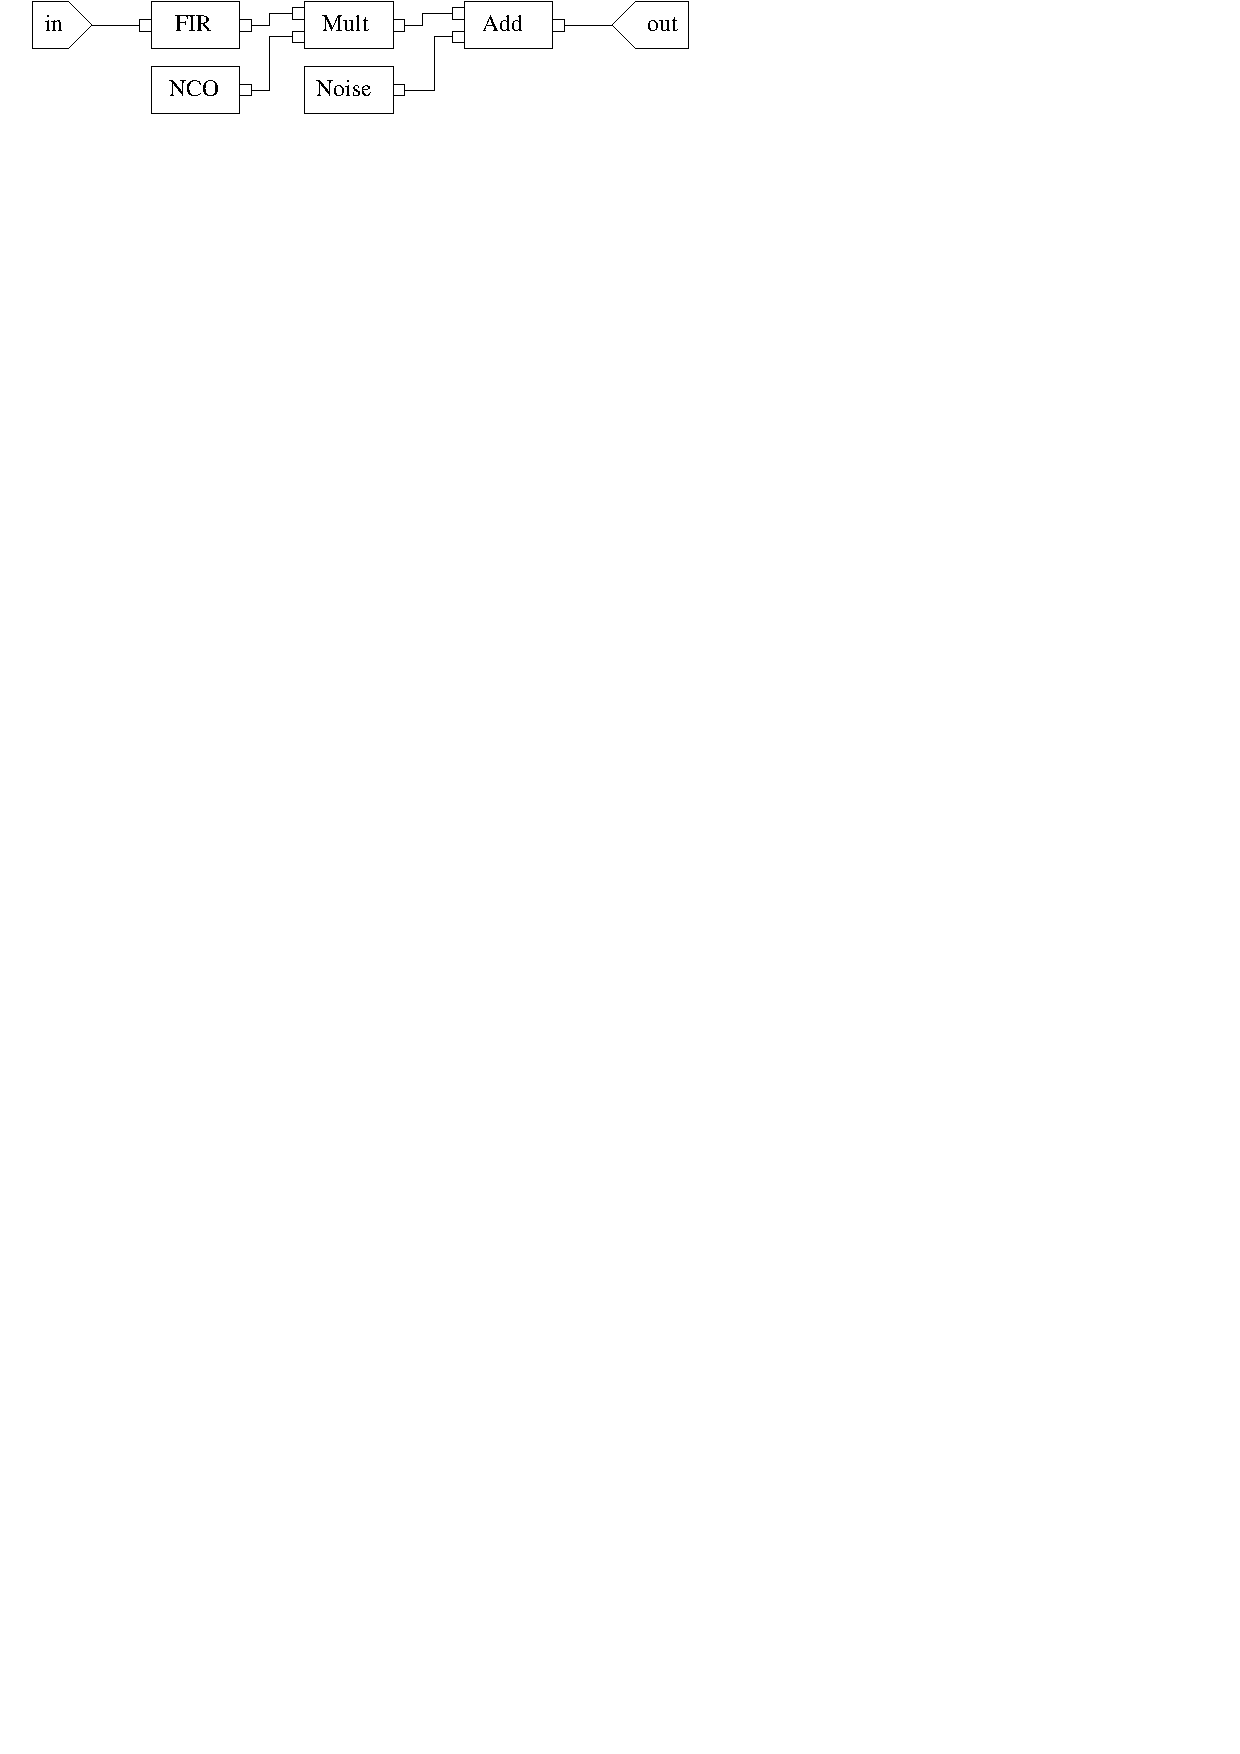
\includegraphics{gralg_example}
\caption{Wireless communication channel simulation model}\label{fig:gralg_example}
\end{figure}

\subsection{An Example: Wireless Channel Simulation}

It will be shown how a model for a static wireless channel can be implemented as a GNU~Radio \textbf{hierarchical} block. The channel is affected by multipath propagation, frequency offset and additive noise. ~\cref{fig:gralg_example} shows a model with internal blocks and corresponding ports \cite{Auras}.

Multipath effects are modeled using a FIR-filter where complex filter coefficients are taken from an arbitrary channel model, e.g., Rayleigh channel model. The signal from an input port is derived to the corresponding GNU~Radio block \textbf{gr.fir\_filter\_ccc}. The suffix ccc denotes that the input stream, output stream and filter coefficients are of complex data types.

According to (\ref{eqn:received_time_freqshift}), the frequency offset is modeled as a sinus wave with fixed frequency and is multiplied with the incoming signal. The corresponding GNU radio blocks are the complex sine signal source \textbf{gr.sig\_source\_c} and the multiplicator with complex inputs and outputs \textbf{gr.multiply\_cc}, respectively.

Finally, complex additive Gaussian noise generated by \textbf{gr.noise\_source\_c} is added to the incoming signal in the \textbf{gr.add\_cc} block and the result is directed to the output port.

The initial parameters of a given hierarchical block, named \textbf{simple\_channel}, are additive noise standard variance, frequency offset normalized to sampling frequency and complex FIR-filter coefficients. IO signatures of input and output ports are identical, and in the framework there is minimum one port and maximum one port for both input and output.

During runtime, internal blocks are initialized and connected to the flowgraph.
The corresponding python\index{Python} script is shown below.
\begin{program}[thb]
\begin{verbatim}
class simple_channel(gr.hier_block2):
  def __init__(self, noise_rms, frequency_offset, channel_coefficients):
    gr.hier_block2.__init__(self, "simple_channel", # Blocktype Identifier
        gr.io_signature(1,1,gr.sizeof_gr_complex),  # incoming
        gr.io_signature(1,1,gr.sizeof_gr_complex))  # outgoing

    # for example channel_coefficients = [0.5+0.1j, 0.2-0.01j]
    multipath_sim = gr.fir_filter_ccc(1, channel_coefficients)

    # frequency_offset normalized to sampling frequency
    # amplitude = 1.0, DC offset = 0.0
    offset_src = gr.sig_source_c(1, gr.GR_SIN_WAVE, frequency_offset, 1.0, 0.0)
    mix = gr.multiply_cc()

    # noise_rms -> var(noise) = noise_rms**2
    noise_src = gr.noise_source_c(gr.GR_GAUSSIAN, noise_rms/sqrt(2))
    add_noise = gr.add_cc()

    # describe signal paths
    self.connect(self, multipath_sim)       # incoming port
    self.connect(multipath_sim, (mix,0))
    self.connect(offset_src, (mix,1))
    self.connect(mix, (noise_add,0))
    self.connect(noise_src, (noise_add,1))
    self.connect(noise_add, self)           # outgoing port
\end{verbatim}
\caption{Python script for simulation of a wireless communication channel}
\end{program}

\section{Installing GNU Radio}

GNU Radio can be run on multiple \glspl{os}, although the most reliable platform is a Linux-based environment, e.g., Ubuntu or Mint.
For Windows and macOS Radioconda can be installed, which bundles a collection of cross-platform installers for numerous open-source software radio packages.

More instructions can be found at \url{https://wiki.gnuradio.org/index.php?title=InstallingGR}. \textbf{Do not} follow the instructions under \textit{Other Installation Methods}. If not clear, contact your lab assistant.






